\chapter{Jupyter}
\section{Introduction}
Jupyter/IPython Notebook Quick Start Guide
This document is a brief step-by-step tutorial on installing and running Jupyter (IPython) notebooks on local computer for new users who have no familiarity with python.

Briefly, if someone gave you a notebook to run and you don’t know what a notebook is, this document is for you.

Jupyter Notebook App (formerly IPython Notebook) is an application running inside the browser. This guide describes how to install and use Jupyter Notebook App as normal desktop application, without using any remote server.

For other use-cases, please refer to the Official Jupyter Documentation.

\section{What is the Jupyter Notebook?}

In this page briefly introduce the main components of the Jupyter Notebook environment. For a more complete overview see References.

\subsection{Notebook document}
Notebook documents (or “notebooks”, all lower case) are documents produced by the Jupyter Notebook App, which contain both computer code (e.g. python) and rich text elements (paragraph, equations, figures, links, etc…). Notebook documents are both human-readable documents containing the analysis description and the results (figures, tables, etc..) as well as executable documents which can be run to perform data analysis.
\subsection{Jupyter Notebook App}
The Jupyter Notebook App is a server-client application that allows editing and running notebook documents via a web browser. The Jupyter Notebook App can be executed on a local desktop requiring no internet access (as described in this document) or can be installed on a remote server and accessed through the internet.

In addition to displaying/editing/running notebook documents, the Jupyter Notebook App has a “Dashboard” (Notebook Dashboard), a “control panel” showing local files and allowing to open notebook documents or shutting down their kernels.

\subsection{kernel}
A notebook kernel is a “computational engine” that executes the code contained in a Notebook document. The ipython kernel, referenced in this guide, executes python code. Kernels for many other languages exist (official kernels).

When you open a Notebook document, the associated kernel is automatically launched. When the notebook is executed (either cell-by-cell or with menu Cell -> Run All), the kernel performs the computation and produces the results. Depending on the type of computations, the kernel may consume significant CPU and RAM. Note that the RAM is not released until the kernel is shut-down.

See also Close a notebook: kernel shut down.

References: from the official docs Opening Notebooks and Decoupled two-process model.

\subsection{Notebook Dashboard}
The Notebook Dashboard is the component which is shown first when you launch Jupyter Notebook App. The Notebook Dashboard is mainly used to open notebook documents, and to manage the running kernels (visualize and shutdown).

The Notebook Dashboard has other features similar to a file manager, namely navigating folders and renaming/deleting files.
Shut down the Jupyter Notebook App
Closing the browser (or the tab) will not close the Jupyter Notebook App. To completely shut it down you need to close the associated terminal.

In more detail, the Jupyter Notebook App is a server that appears in your browser at a default address (http://localhost:8888). Closing the browser will not shut down the server. You can reopen the previous address and the Jupyter Notebook App will be redisplayed.

You can run many copies of the Jupyter Notebook App and they will show up at a similar address (only the number after “:”, which is the port, will increment for each new copy). Since with a single Jupyter Notebook App you can already open many notebooks, we do not recommend running multiple copies of Jupyter Notebook App.

\subsection{Close a notebook: kernel shut down}
When a notebook is opened, its “computational engine” (called the kernel) is automatically started. Closing the notebook browser tab, will not shut down the kernel, instead the kernel will keep running until is explicitly shut down.

To shut down a kernel, go to the associated notebook and click on menu File -> Close and Halt. Alternatively, the Notebook Dashboard has a tab named Running that shows all the running notebooks (i.e. kernels) and allows shutting them down (by clicking on a Shutdown button).

\section{Notebook Basics}
\subsection{The Notebook dashboard}
When you first start the notebook server, your browser will open to the notebook dashboard. The dashboard serves as a home page for the notebook. Its main purpose is to display the notebooks and files in the current directory. For example, here is a screenshot of the dashboard page for the examples directory in the Jupyter repository:

\begin{figure}
    \centering
    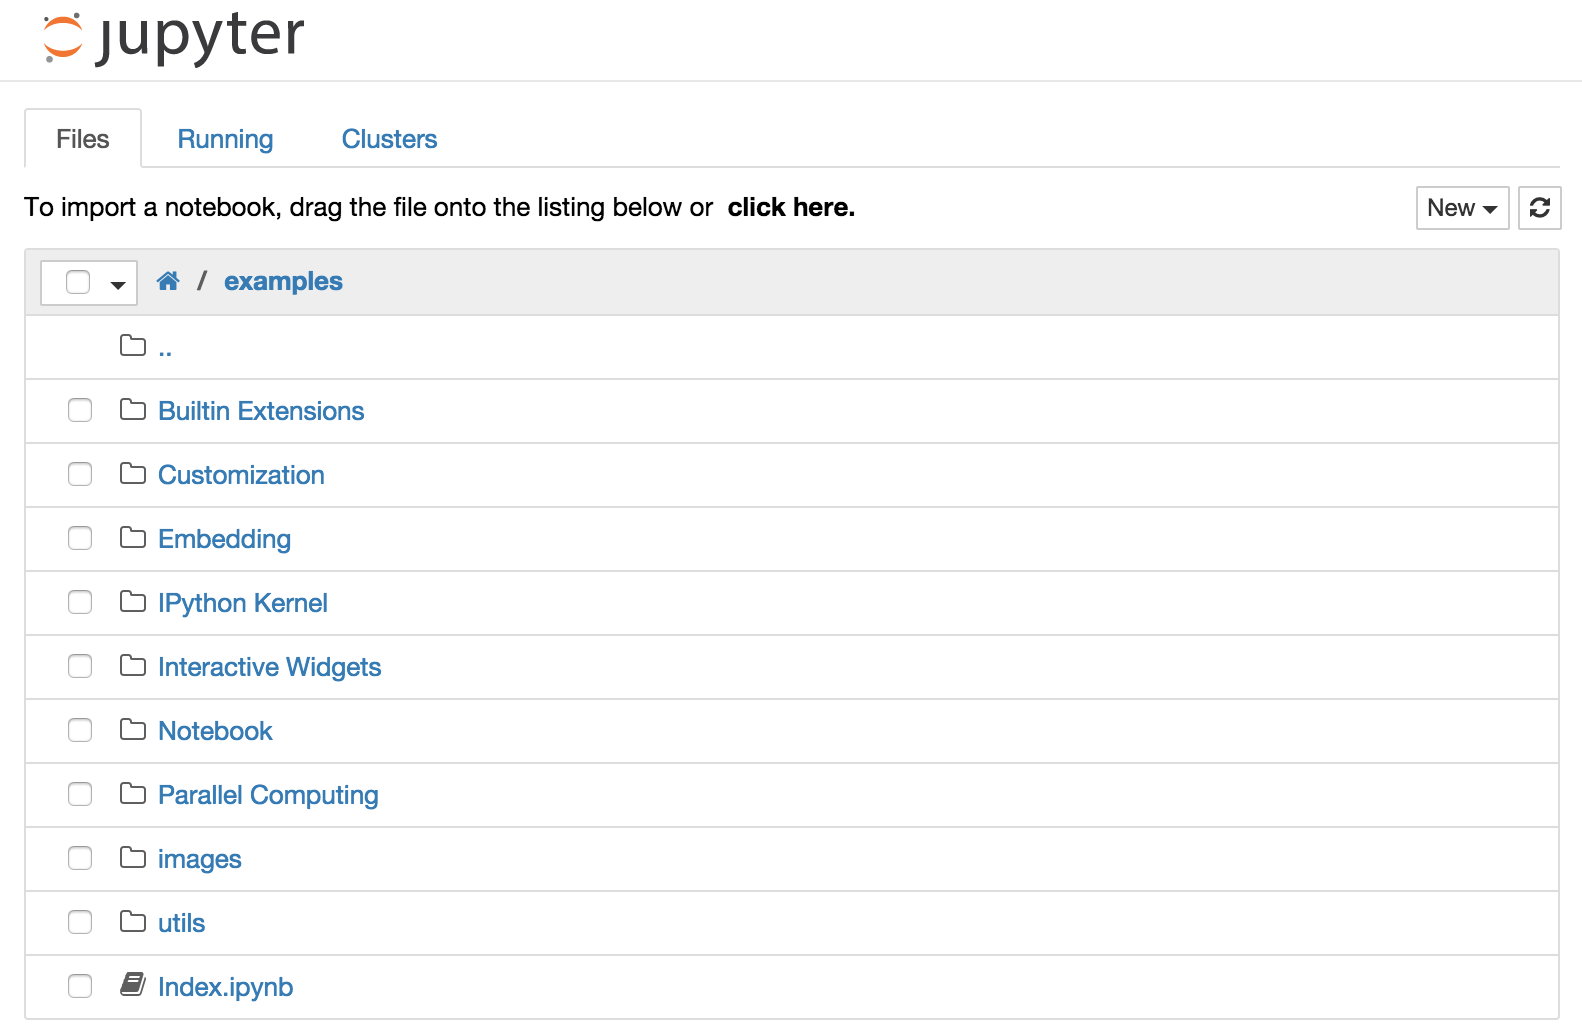
\includegraphics[width=\linewidth]{dashboard_files_tab.png}
\end{figure}

The top of the notebook list displays clickable breadcrumbs of the current directory. By clicking on these breadcrumbs or on sub-directories in the notebook list, you can navigate your file system.\\

To create a new notebook, click on the "New" button at the top of the list and select a kernel from the dropdown (as seen below). Which kernels are listed depend on what's installed on the server. Some of the kernels in the screenshot below may not exist as an option to you.

\begin{marginfigure}
    \centering
    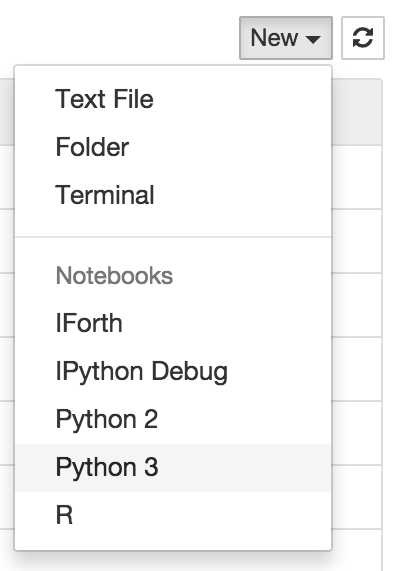
\includegraphics[]{dashboard_files_tab_new.png}
\end{marginfigure}

Notebooks and files can be uploaded to the current directory by dragging a notebook file onto the notebook list or by the "click here" text above the list.

The notebook list shows green "Running" text and a green notebook icon next to running notebooks (as seen below). Notebooks remain running until you explicitly shut them down; closing the notebook's page is not sufficient.

\begin{figure}
    \centering
    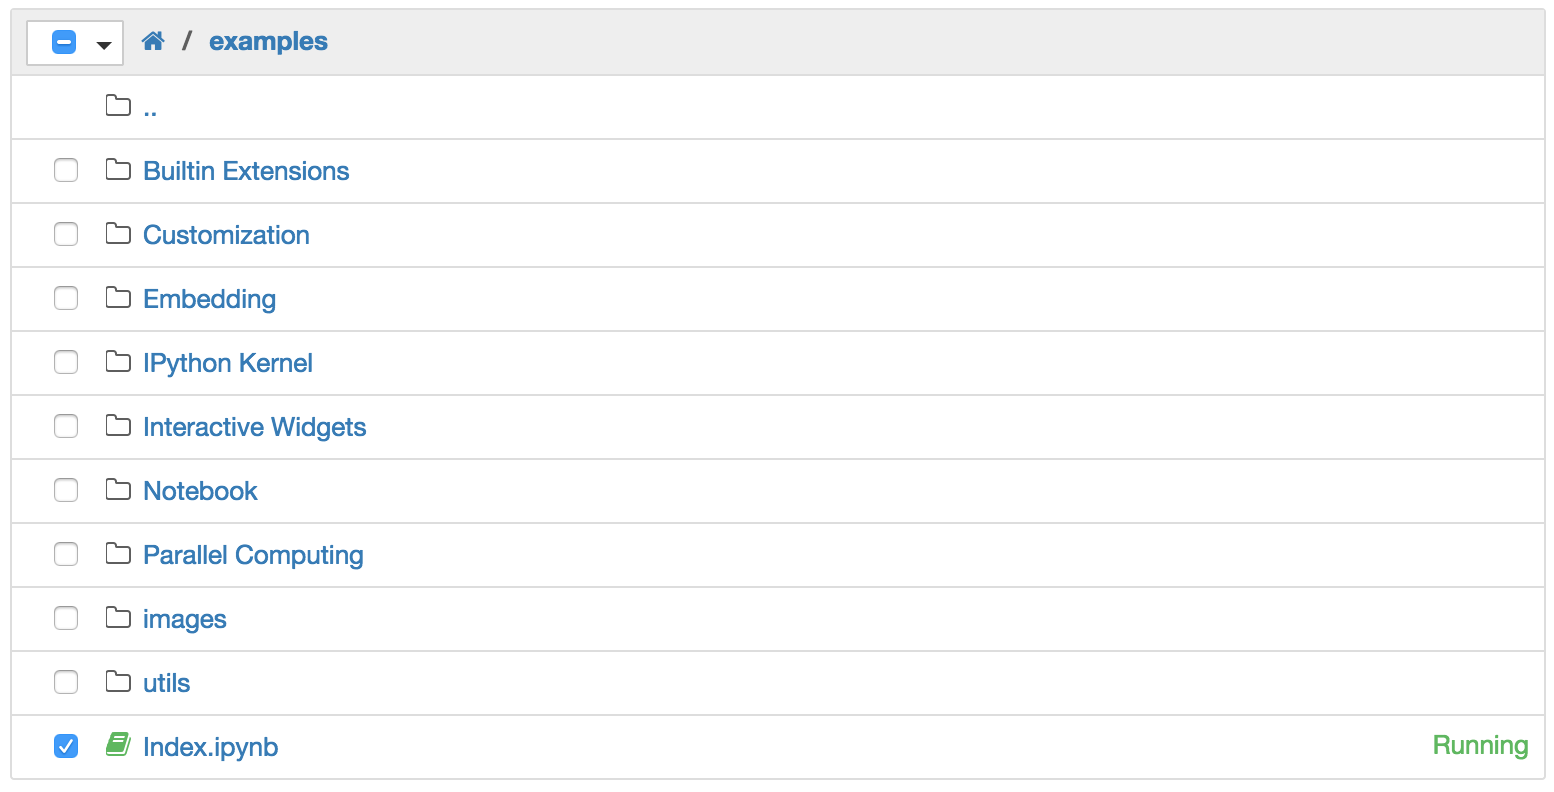
\includegraphics[width=0.5\linewidth]{dashboard_files_tab_run.png}
\end{figure}

To shutdown, delete, duplicate, or rename a notebook check the checkbox next to it and an array of controls will appear at the top of the notebook list (as seen below). You can also use the same operations on directories and files when applicable.

\begin{figure}
    \centering
    
\includegraphics[width=0.5\linewidth]{dashboard_files_tab_btns.png}
\end{figure}

To see all of your running notebooks along with their directories, click on the "Running" tab:

\begin{figure}
    \centering
    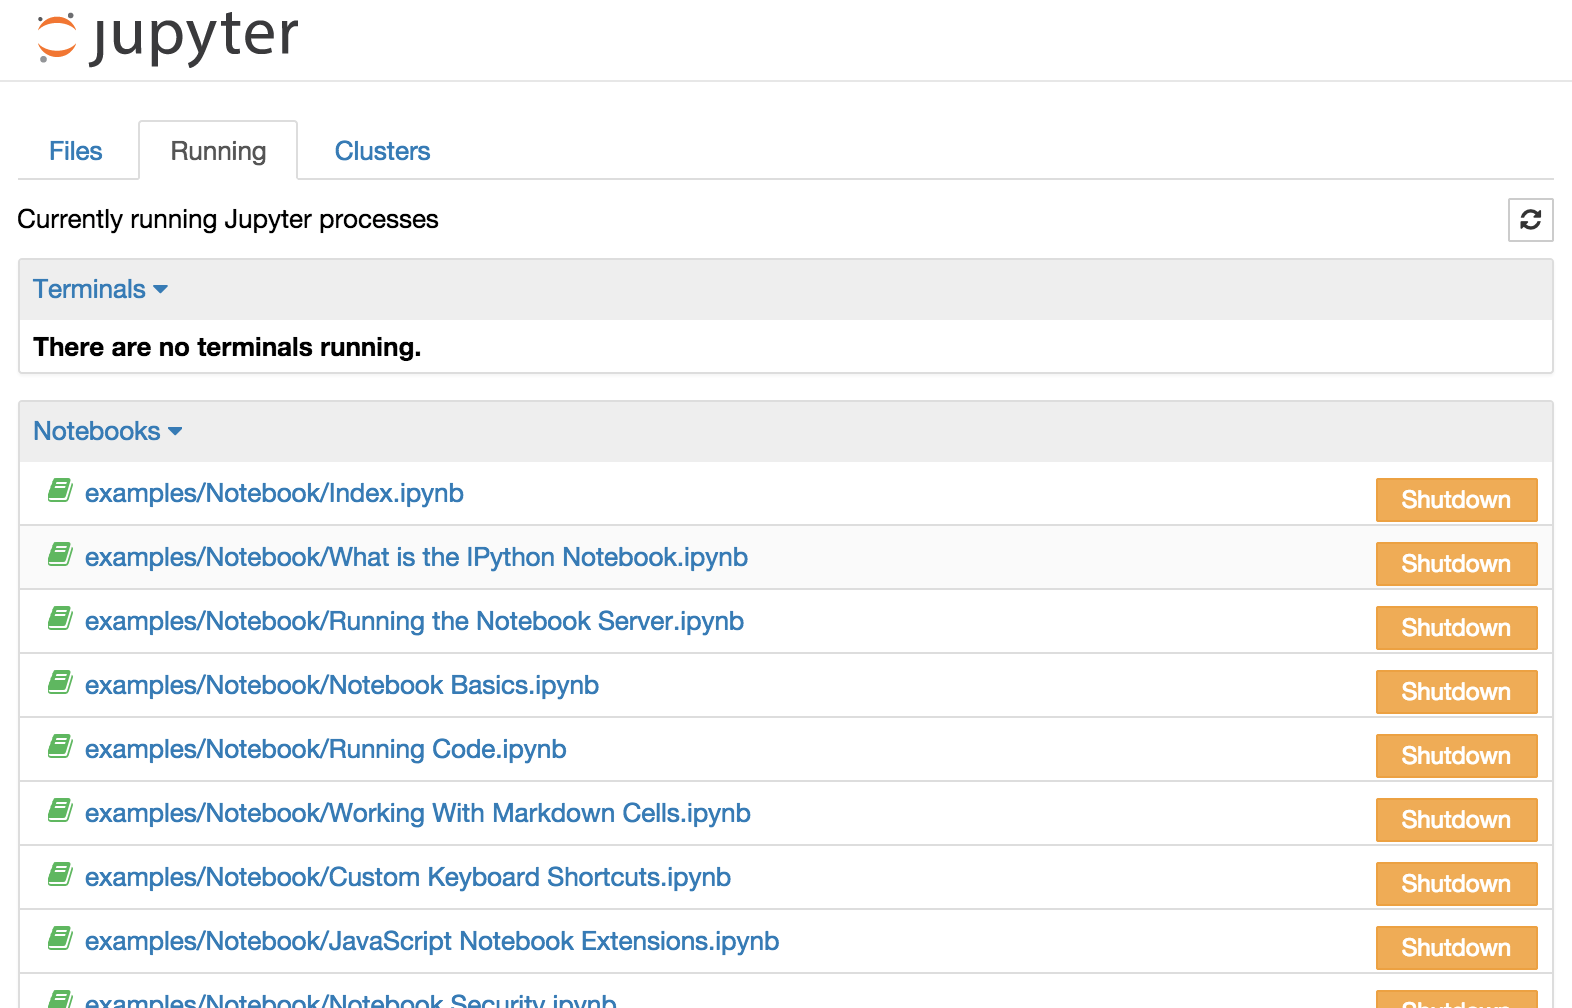
\includegraphics[width=0.5\linewidth]{dashboard_running_tab.png}
\end{figure}

This view provides a convenient way to track notebooks that you start as you navigate the file system in a long running notebook server.

Overview of the Notebook UI
If you create a new notebook or open an existing one, you will be taken to the notebook user interface (UI). This UI allows you to run code and author notebook documents interactively. The notebook UI has the following main areas:

\titem Menu
\titem Toolbar
\titem Notebook area and cells
The notebook has an interactive tour of these elements that can be started in the "Help:User Interface Tour" menu item.

\subsection{Modal editor}
Starting with IPython 2.0, the Jupyter Notebook has a modal user interface. This means that the keyboard does different things depending on which mode the Notebook is in. There are two modes: edit mode and command mode.

\subsection{Edit mode}
Edit mode is indicated by a cell border and a prompt showing in the editor area:

\begin{figure}
    \centering
    
\includegraphics[width=0.5\linewidth]{edit_mode.png}
\end{figure}

When a cell is in edit mode, you can type into the cell, like a normal text editor.

Enter edit mode by pressing `Enter` or using the mouse to click on a cell's editor area.
In this mode you can change the type of cell with the dropdown menu:  
\begin{figure}
    \centering
    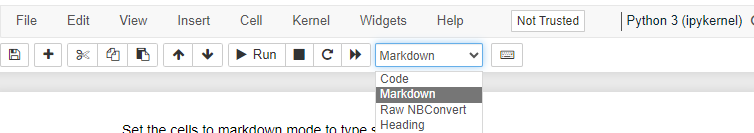
\includegraphics[width=0.5\linewidth]{celltype.png}
\end{figure}

A \emph{markdown cell} allows you to type and format text using the markdown 


\subsection{Command mode}
Command mode is indicated by a grey cell border with a blue left margin:

\begin{figure}
    \centering
    
\includegraphics[width=0.5\linewidth]{command_mode.png}
\end{figure}

When you are in command mode, you are able to edit the notebook as a whole, but not type into individual cells. Most importantly, in command mode, the keyboard is mapped to a set of shortcuts that let you perform notebook and cell actions efficiently. For example, if you are in command mode and you press c, you will copy the current cell - no modifier is needed.

Don't try to type into a cell in command mode; unexpected things will happen!
Enter command mode by pressing `Esc` or using the mouse to click *outside* a cell's editor area.

\subsection{Mouse navigation}
All navigation and actions in the Notebook are available using the mouse through the menubar and toolbar, which are both above the main Notebook area:

\begin{figure}
    \centering
    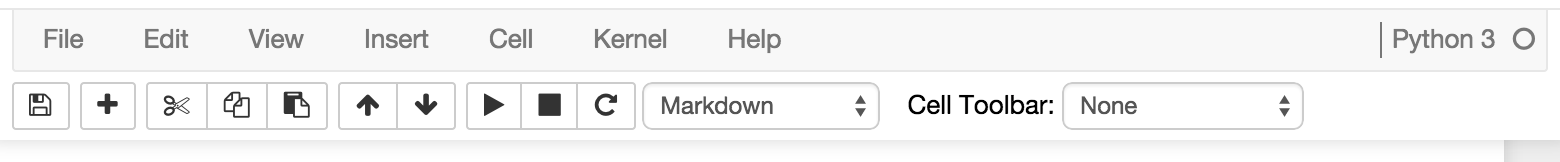
\includegraphics[width=0.5\linewidth]{menubar_toolbar.png}
\end{figure}

The first idea of mouse based navigation is that cells can be selected by clicking on them. The currently selected cell gets a grey or green border depending on whether the notebook is in edit or command mode. If you click inside a cell's editor area, you will enter edit mode. If you click on the prompt or output area of a cell you will enter command mode.\\

If you are running this notebook in a live session (not on https://nbviewer.jupyter.org) try selecting different cells and going between edit and command mode. Try typing into a cell.\\

The second idea of mouse based navigation is that cell actions usually apply to the currently selected cell. Thus if you want to run the code in a cell, you would select it and click the button in the toolbar or the "Cell:Run" menu item. Similarly, to copy a cell you would select it and click the button in the toolbar or the "Edit:Copy" menu item. With this simple pattern, you should be able to do most everything you need with the mouse.\\

Markdown cells have one other state that can be modified with the mouse. These cells can either be rendered or unrendered. When they are rendered, you will see a nice formatted representation of the cell's contents. When they are unrendered, you will see the raw text source of the cell. To render the selected cell with the mouse, click the button in the toolbar or the "Cell:Run" menu item. To unrender the selected cell, double click on the cell.\\

\section{Keyboard Navigation}
The modal user interface of the Jupyter Notebook has been optimized for efficient keyboard usage. This is made possible by having two different sets of keyboard shortcuts: one set that is active in edit mode and another in command mode.

The most important keyboard shortcuts are Enter, which enters edit mode, and Esc, which enters command mode.

In edit mode, most of the keyboard is dedicated to typing into the cell's editor. Thus, in edit mode there are relatively few shortcuts. In command mode, the entire keyboard is available for shortcuts, so there are many more. The Help->Keyboard Shortcuts dialog lists the available shortcuts.
\subsection{Shortcuts}
I recommend learning the command mode shortcuts in the following rough order:

Basic navigation: enter, shift-enter, up/k, down/j\\
Saving the notebook: s\\
Change Cell types: y, m, 1-6, t\\
Cell creation: a, b\\
Cell editing: x, c, v, d, z\\
Kernel operations: i, 0 (press twice)\\

\chapter{Conducting a practical}

Lets see how the previous chapter works in practice. To begin with we open a new jupyter file and name it sensibly:\\
\begin{figure}
    \centering
    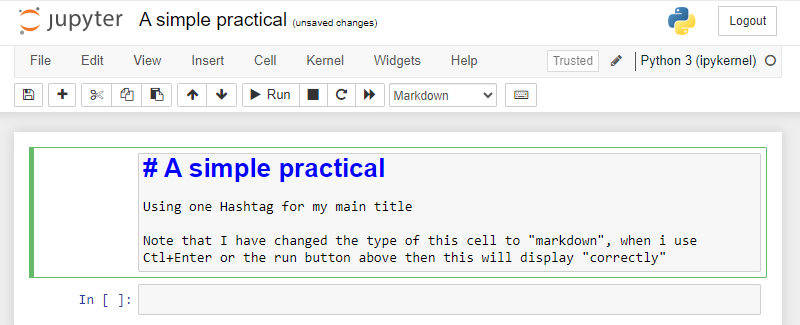
\includegraphics[width=1\linewidth]{figures/SimplePrac.png}
\end{figure}
Then we start to add the detail\sidenote[][]{All practical work should contain: \begin{itemize} \item Title\\ \item Apparatus list and/or set-up diagram and commentary on why you have chosen the equipment. eg. Using a $\pm 0.001$mm micrometer would give you appropriate precision for measuring a thin wire\\ \item A method with appropriate safety precautions (this needn't be longer than "set up as in diagram" for some practicals!)\\ \item A results table\\ \item A concluding statement\\ \end{itemize}}: 
\begin{figure}
    \centering
    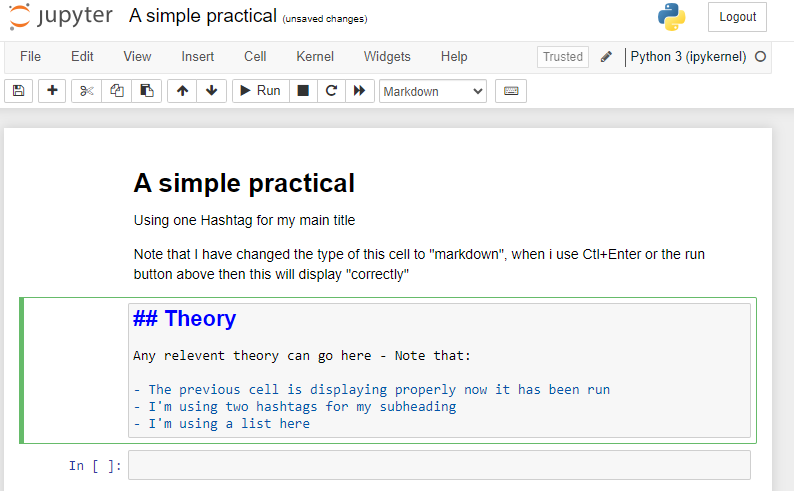
\includegraphics[width=1\linewidth]{figures/theoryprac.png}
\end{figure}
I've added an image by finding a good one online, saving it, and dragging and dropping it to the cell:\\
\begin{figure}[h!]
    \centering
    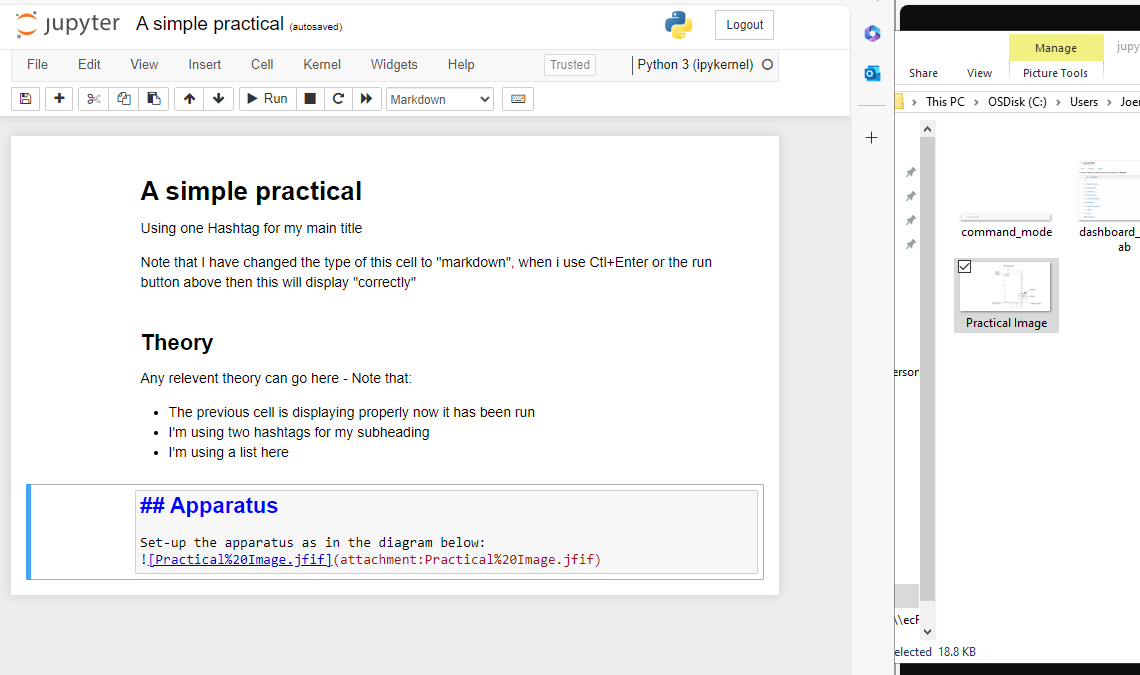
\includegraphics[width=1\linewidth]{figures/pracimage.png}
\end{figure}
Now we're into the code for your results etc. Some commented code explaining the function of each bit follows. A sensible student would use a basic version of this as a boilerplate (a partially complete template version) for all of your future write-ups.\\ 

\begin{figure}[h!]
    \centering
    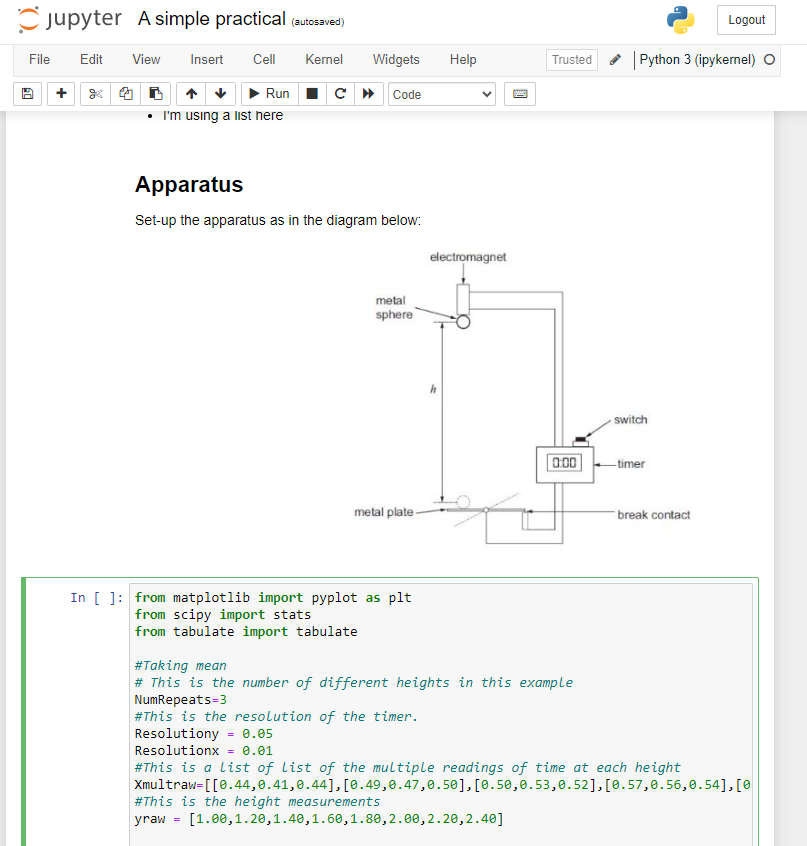
\includegraphics[width=1\linewidth]{figures/praccode.png}
\end{figure}
\newpage
\subsection{Example code for your results}

This code is for the "g by freefall" experiment in which a ball is dropped, it's time of flight timed, and the acceleration due to gravity calculated.

\begin{fullwidth}
    

\begin{mintedbox}{python}
from matplotlib import pyplot as plt
from scipy import stats
from tabulate import tabulate

#Taking mean
# This is the number of different heights in this example
NumRepeats=3
#This is the resolution of the timer. 
Resolutiony = 0.05
Resolutionx = 0.01
#This is a list of list of the multiple readings of time at each height
Xmultraw=[[0.44,0.41,0.44],[0.49,0.47,0.50],[0.50,0.53,0.52],[0.57,0.56,0.54],[0.60,0.62,0.59],
[0.61,0.66,0.63],[0.67,0.67,0.67],[0.70,0.70,0.70]]
#This is the height measurements
yraw = [1.00,1.20,1.40,1.60,1.80,2.00,2.20,2.40]


# Looping over the number of heights. Calculating the average time and the uncertainty in those times and adding them to the 
# list xraw and uncertainty
xraw=[]
uncertaintyxraw=[]
for i in range (len(yraw)):
    sumx=0.0
    for j in range (NumRepeats):
        sumx+=Xmultraw[i][j]        
    HalfRange=(max(Xmultraw[i])-min(Xmultraw[i]))/2.0
    ave=sumx/NumRepeats
    if HalfRange < Resolutionx:
        HalfRange=Resolutionx
    uncertaintyxraw.append(HalfRange)
    xraw.append(ave)

# looping over the length of y and calculation 2h and t^2 so that the correct thing is plotted against each other
y=[]
x=[]
uncertaintyx=[]
uncertaintyy=[]
for i in range (len(xraw)):
    y.append(2*yraw[i])
    x.append(xraw[i]*xraw[i])
    uncertaintyx.append(2.0*(uncertaintyxraw[i]/xraw[i])*x[i])
    uncertaintyy.append(Resolutiony*2)

# merging the varaiables into one list of lists so tht tabulate can cope
merged_list = [(y[i],*Xmultraw[i],xraw[i],uncertaintyxraw[i],x[i],uncertaintyx[i]) for i in range (0,len(x))]
labels=['2 x h (m)','Time 1 (s)','Time 2 (s)','Time 3 (s)','Mean t (s)', 'unc t (s)', 'Mean t^2 (s)','unc t^2 (s^2)']
print(tabulate(merged_list, headers=labels,tablefmt='fancy_grid',floatfmt=".2f"))
\end{mintedbox}

Having run the code, it prints us a lovely table of results. Note that it displays the calculated means, some uncertainty and the calculated values of $t^2$. Note also that the table has headings with units for each column: 
\begin{figure}
    \centering
    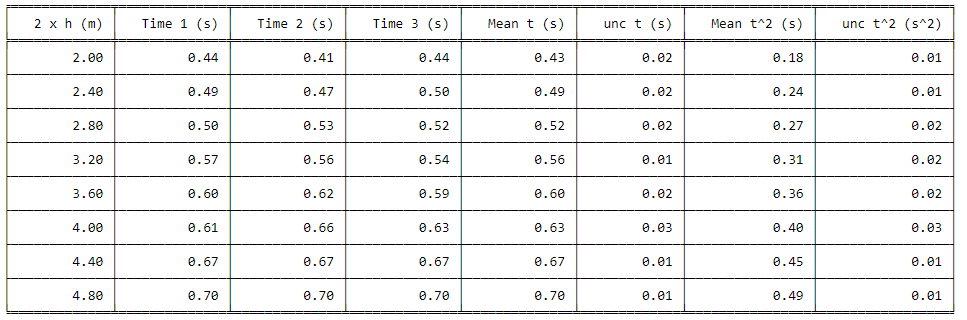
\includegraphics[width=1\linewidth]{figures/resultstable.png}
\end{figure}
\end{fullwidth}
With the results taken and processed, it's time to do some analysis. In A-Level physics terms this means that we need to plot a graph, draw a line of best fit (a linear regression), and almost always - calculate a gradient. There are a few practicals where we draw non-linear relationships, or have no graph at all, but they are generally few and far between. 

For the results above, the perfect graph will look something like this\footnote{It's really important to realise - if you're reading this in Y12 - that youdon't need to learn all of this at once. We will learn this coding together}: 
\begin{figure}
    \centering
    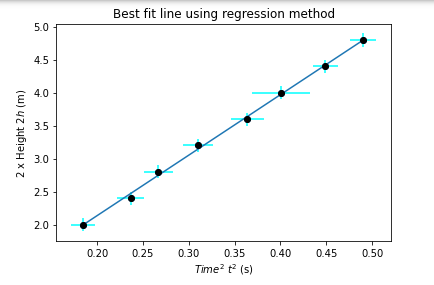
\includegraphics[width=1\linewidth]{figures/graphper.png}
\end{figure}

\begin{fullwidth}
\begin{mintedbox}{python}
from scipy import stats
# Calling linear regression assigning the output to the variables on the left of the equation 
gradient, intercept,r,p,st_err = stats.linregress(x,y)
#looping over the length of x and applying y=mx+c using the m and c from the output above to find the regression line   
line=[]
for i in range (len(x)):
    line.append(gradient*x[i]+intercept)
# Plotting the data points and the best fit line
plt.scatter(x, y)
plt.errorbar(x,y,xerr=uncertaintyx,yerr=uncertaintyy,fmt='o',ecolor='cyan', color='black')
plt.plot(x,line)
plt.title('Best fit line using regression method')
plt.ylabel('2 x Height $2h$ (m)')
plt.xlabel('$Time^2$ $t^2$ (s)')

plt.show()
print ("Gradient=%.2f"%gradient,'ms-2')
print("Our y intercept should be zero it is equal to = ",intercept)
\end{mintedbox}
\end{fullwidth}
The output of this code is the above graph, but it will also print a gradient and intercept value: 
\begin{verbatim}
Gradient=9.18 ms-2
Our y intercept should be zero it is equal to =  0.29863797357735233  
\end{verbatim}

\section{Conclusions}
The final part of any practical write-up is the concluding statement. For this practical it would look like this:

\begin{fullwidth}
    \begin{mintedbox}{python}
print('Our calculated value of %.2f m/s^2 is close the value stated in our data booklet of 9.81 m/s^2' %gradient)
print('The line of best fit goes through all the error bars. This means we have verified the law and found a reasonable value of g.')
    \end{mintedbox}
\end{fullwidth}
We have done a few important things here:
\titem We have compared our value to a known value.
\titem We have quoted the source of information for the known value.
\titem We have concluded with a comment on the quality of our data and the implications of our experiment.

\newpage
\section{A complete example}
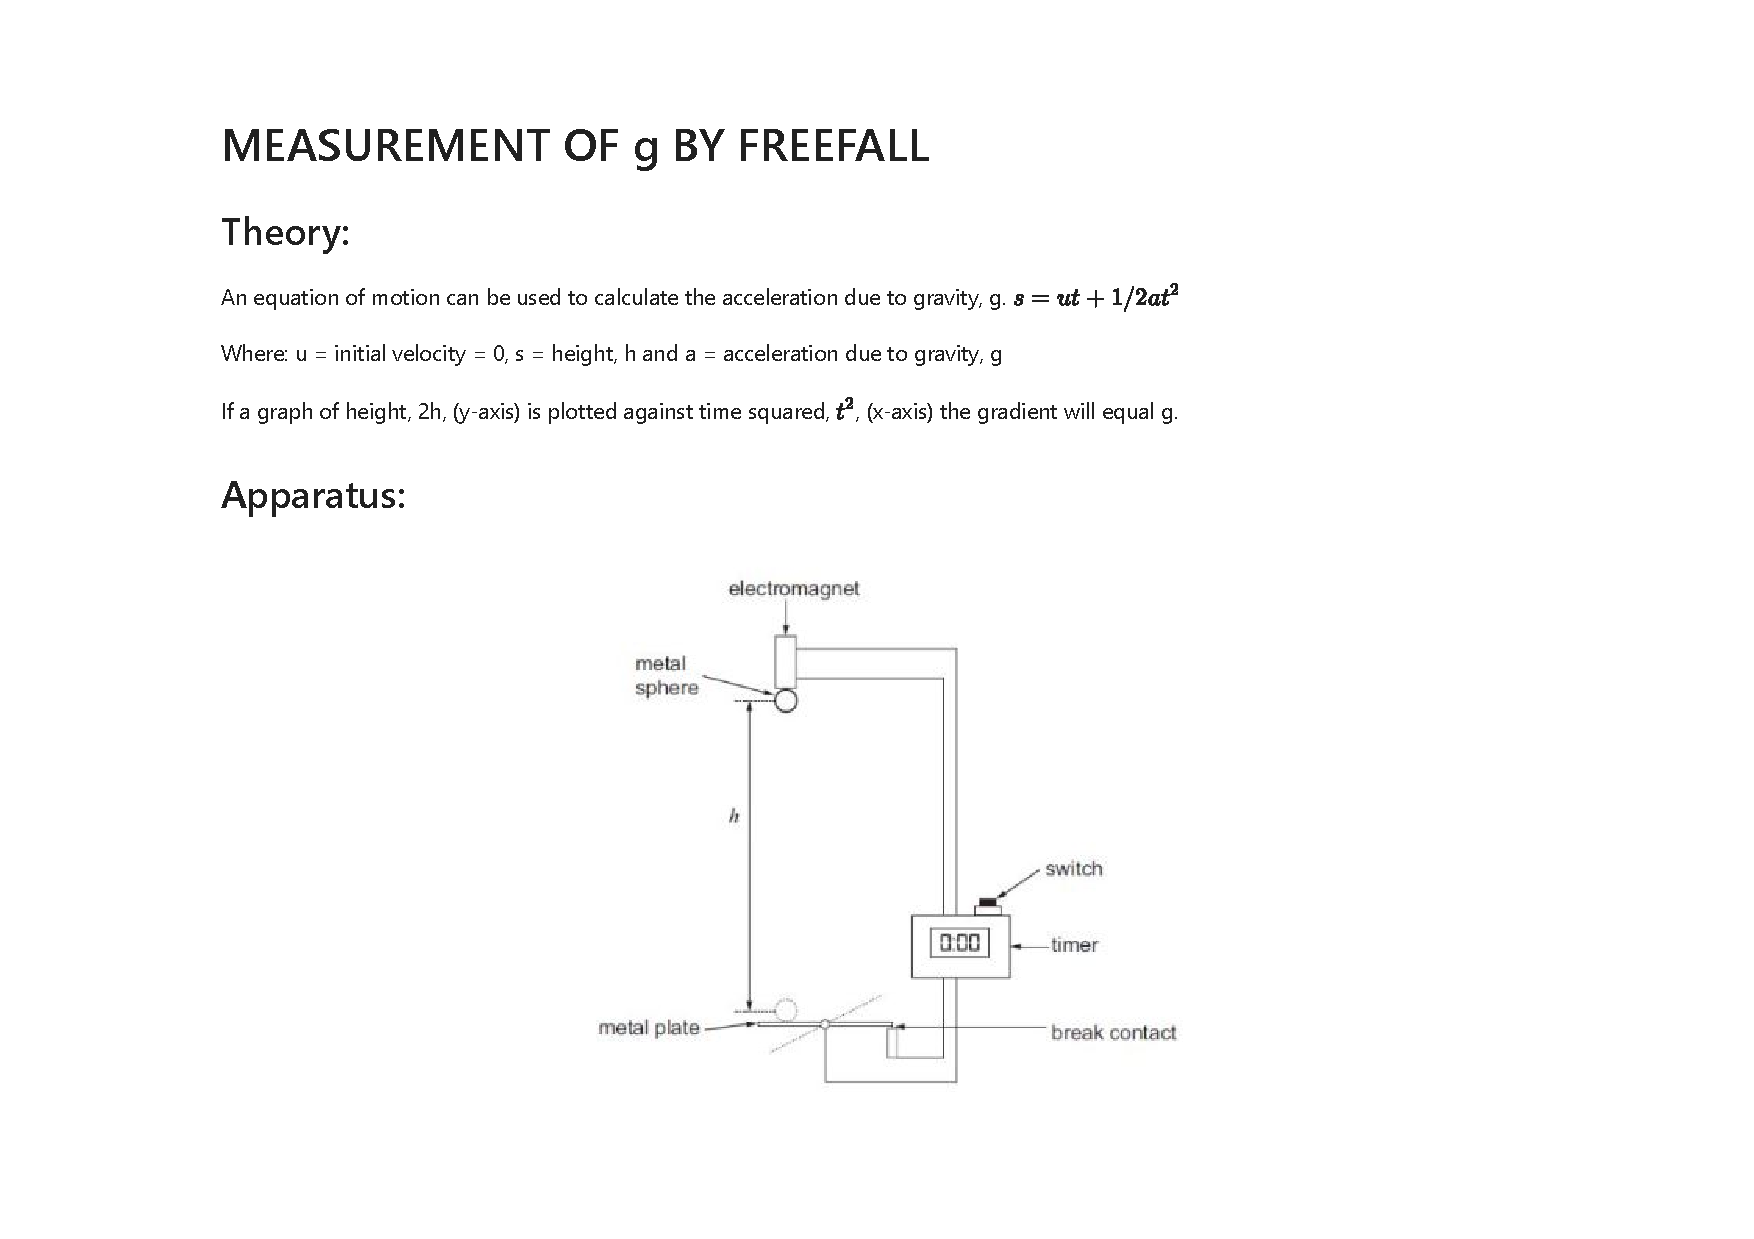
\includepdf[pages=-,nup=1x2]{fullprac.pdf}

\chapter{Markdown Guide}


You can use Markdown to format documentation you add to Markdown cells in your Jupyter notebook.

Here's how to format Markdown cells in Jupyter notebooks:

\subsection{Headings:}

Use the number sign (\#) followed by a blank space for notebook titles and section headings:
\begin{verbatim}    
# for titles
## for major headings
### for subheadings
#### for 4th level subheadings
\end{verbatim}

\subsection{Emphasis}
Use the following code to emphasize text:
\begin{verbatim}

Bold text: __string__ or **string**
Italic text: _string_ or *string*
\end{verbatim}

\section{Mathematical symbols}
Surround mathematical symbols with a dollar sign (\$), for example:
\begin{verbatim}
    $ mathematical symbols $
\end{verbatim}

\section{Monospace font}
Surround text with a grave accent (`) also called a back single quotation mark, for example:
\begin{verbatim}
    `string`
\end{verbatim}

You can use the monospace font for file paths, file names, message text that users see, or text that users enter.

\section{Line breaks}
Sometimes markdown doesn’t make line breaks when you want them. To force a linebreak, use the following code: \begin{verbatim}
    <br>
\end{verbatim}

\section{Indenting}
Use the greater than sign (>) followed by a space, for example:
\begin{verbatim}
> Text that will be indented when the Markdown is rendered. 
\end{verbatim}
Any subsequent text is indented until the next carriage return.

\section{Bullets}
To create a circular bullet point, use one of the following methods. Each bullet point must be on its own line.
A hyphen (-) followed by one or two spaces, for example: - Bulleted item
A space, a hyphen (-) and a space, for example: - Bulleted item
An asterisk (*) followed by one or two spaces, for example: * Bulleted item
To create a sub bullet, press Tab before entering the bullet point using one of the methods described above. For example:
- Main bullet point
     - Sub bullet point

\section{Numbered lists}
To create a numbered list, enter 1. followed by a space, for example:
\begin{verbatim}
1. Numbered item
1. Numbered item   
\end{verbatim}

For simplicity, you use 1. before each entry. The list will be numbered correctly when you run the cell.

To create a substep, press Tab before entering the numbered item, for example:
\begin{verbatim}
    1. Numbered item
     1. Substep
\end{verbatim}

\section{Colored note boxes}
Use one of the following <div> tags to display text in a colored box.
Restriction: Not all Markdown code displays correctly within <div> tags, so review your colored boxes carefully.\\
For example, to make a word bold, surround it with the HTML code for bold (<b>text</b> instead of the Markdown code.\\
The color of the box is determined by the alert type that you specify:
\subsection{Blue boxes (alert-info)}
\begin{verbatim}
   
<div class="alert alert-block alert-info">
<b>Tip:</b> Use blue boxes (alert-info) for tips and notes. 
If it’s a note, you don’t have to include the word “Note”.
</div> 
\end{verbatim}
\subsection{Yellow boxes (alert-warning)}
\begin{verbatim}
   
<div class="alert alert-block alert-warning">
<b>Example:</b> Use yellow boxes for examples that are not 
inside code cells, or use for mathematical formulas if needed.
</div> 
\end{verbatim}


\subsection{Green boxes (alert-success)}
\begin{verbatim}
  <div class="alert alert-block alert-success">
<b>Up to you:</b> Use green boxes sparingly, and only for some specific 
purpose that the other boxes can't cover. For example, if you have a lot 
of related content to link to, maybe you decide to use green boxes for 
related links from each section of a notebook.
</div>  
\end{verbatim}

\subsection{Red boxes (alert-danger)}
\begin{verbatim}
    
<div class="alert alert-block alert-danger">
<b>Just don't:</b> In general, avoid the red boxes. These should only be
used for actions that might cause data loss or another major issue.
</div>
\end{verbatim}

\section{Graphics}
You can attach image files directly to a notebook in Markdown cells by dragging and dropping it into the cell.
To add images to other cell types, use graphics that are hosted on the web with this code, substituting url/name with the full URL and name of the image:
\begin{verbatim}
<img src=“url/filename.gif” alt=“Alt text” title=“Title text” />
\end{verbatim}
Restriction: You cannot add captions to graphics.
\section{Geometric shapes}
Use \&\# followed by the decimal or hex reference number for the shape, for example:
\begin{verbatim}
 &#reference_number   
\end{verbatim}

For a list of reference numbers, see UTF-8 Geometric shapes.

\subsection{Horizontal lines}
On a new line, enter three asterisks:
\begin{verbatim}
    ***
\end{verbatim}

Internal links
To link to a section within your notebook, use the following code:
\begin{verbatim}
   [Section title](#section-title) 
\end{verbatim}

For the text inside the parentheses, replace any spaces and special characters with a hyphen. For example, if your section is called Analyzing customer purchasing habits, you'd enter:
\begin{verbatim}
  [Analyzing customer purchasing habits](#analyzing-customer-purchasing-habits)  
\end{verbatim}


Alternatively, you can add an ID above the section:
\begin{verbatim}
    <a id="section_ID"></a>
\end{verbatim}

Important: Each ID in the notebook must be unique.
To link to a section that has an ID, use the following code:
\begin{verbatim}
  [Section title](#section_ID)  
\end{verbatim}


Important: Test all internal links to ensure that they work.
External links
To link to an external site, use the following code:
\begin{verbatim}
    __[link text](http://url)__
\end{verbatim}

Surround the link with two underscores on each side

